\documentclass[11pt]{article}
\usepackage{amssymb}
\usepackage{setspace}
\usepackage[british]{babel}
\usepackage[mathscr]{euscript}
\usepackage{graphicx,stmaryrd}
\usepackage{dsfont}
\usepackage{tikz}
\usepackage{amsmath}
\usepackage{amsfonts}
\usepackage{amsthm}
\usepackage{algorithm}
\usepackage{algcompatible}
\usepackage[noend]{algpseudocode}
\usepackage{tikz}
\usepackage[bottom=2.5cm, top = 2.5cm, left = 3cm, right = 2cm]{geometry}
\usepackage{hyperref}
\usetikzlibrary{trees}
\hypersetup{
    colorlinks=true,
    linkcolor=blue,
    urlcolor=blue,
    linktoc=all,
    citecolor=blue
           }
\usepackage{cite}
\onehalfspacing
\setlength\parskip{0.2cm}
\setlength\parindent{0pt}


\newcommand{\R}{\mathbb{R}}
\newtheorem{definition}{Definition}
\newtheorem{axiom}{Axiom}
\newtheorem{lemma}{Lemma}
\newtheorem{theorem}{Theorem}
\newtheorem{proposition}{Proposition}
\newtheorem{corollary}{Corollary}
%\newtheorem{hypothese}{Assumption}
\newtheorem{remark}{Remark}

\newtheorem{innerassumption}{Assumption}
\newenvironment{Assumption}[1]
  {\renewcommand\theinnerassumption{#1}\innerassumption}
  {\endinnerassumption}
  
\makeatletter
\renewenvironment{proof}[1][\proofname]{\par
\pushQED{\qed}%
\normalfont \topsep6\p@\@plus6\p@\relax
\trivlist
\item\relax
{\textbf{
#1\@addpunct{ }}}\hspace\labelsep\ignorespaces
}{%
\popQED\endtrivlist\@endpefalse
}
\makeatother

% Default fixed font does not support bold face
\DeclareFixedFont{\ttb}{T1}{txtt}{bx}{n}{12} % for bold
\DeclareFixedFont{\ttm}{T1}{txtt}{m}{n}{12}  % for normal

% Custom colors
\usepackage{color}
\definecolor{deepblue}{rgb}{0,0,0.5}
\definecolor{deepred}{rgb}{0.6,0,0}
\definecolor{deepgreen}{rgb}{0,0.5,0}
\definecolor{khaki(html/css)(khaki)}{rgb}{0.76, 0.69, 0.57}

\usepackage{listings}

% Python style for highlighting
\newcommand\pythonstyle{\lstset{
language=Python,
basicstyle=\ttm,
morekeywords={self},              % Add keywords here
keywordstyle=\ttb\color{khaki(html/css)(khaki)},
emph={MyClass,__init__},          % Custom highlighting
emphstyle=\ttb\color{deepred},    % Custom highlighting style
stringstyle=\color{deepred},                         % Any extra options here
showstringspaces=false
}}

\newcommand{\indep}{\perp \!\!\! \perp}


% Python environment
\lstnewenvironment{python}[1][]
{
\pythonstyle
\lstset{#1}
}
{}

% Python for external files
\newcommand\pythonexternal[2][]{{
\pythonstyle
\lstinputlisting[#1]{#2}}}

% Python for inline
\newcommand\pythoninline[1]{{\pythonstyle\lstinline!#1!}}

%\renewcommand{\thesection}{\arabic{section}}
\renewcommand{\thefigure}{\arabic{figure}}

\begin{document}
	\section{Introduction}
	Multivariate extremes arise when one or more of rare extremes events occur simultaneously. These events are of prime interest to assess natural hazard stemming from heavy rainfall, wind storms and earthqueakes since they are driven by joint extremes if a number meteorologial variables. It is well known from the classical theory that multivariate distributions can be decomposed into two distinct parts : the analysis of marginal distributions and the analysis of the dependence structure described by the copula function. Results from the extreme-value theory show that the possible dependence structures of extremes have to satisfy certain constraints. Indeed, the possible dependence structure may be described in various equivalent ways (\cite{resnick2008extreme, beirlant2004statistics, de2006extreme}) : by the exponent measure $\Lambda$ (\cite{balkema1977max}), by the Pickands dependence function $A$ (\cite{pickands1981multivariate}), by the stable tail dependence function $L$ (\cite{huang1992statistics}), by the madogram (\cite{naveau2009modelling}), by the extreme value copula $C$ (\cite{gudendorf2010}). Estimating this extreme value copula is an important subject of the extreme litterature see, \emph{e.g.} \cite{bucher2011new, gudendorf2012nonparametric, MARCON20171, escobar2018local} to name a few.
	
	The dependence structure between extreme observations can be complex and characterized by different notions from the ones arises in the classical theory. For this reason, recent works bring various notions to the framework of extreme such as sparsity (\cite{goix2015learning, simpson2020determining, meyer2021sparse}), conditional independence and graphical models (\cite{gissibl2018max, engelke2020graphical, segers2020one}), dimensionality reduction (\cite{chautru2015dimension, drees2021principal}) and unsupervised learning (\cite{cooley2019decompositions, janssen2020k}). In this work, we are concerned about variable clustering as a tool for learning the dependence structure of multivariate extreme and bridge important ideas from modern statistics and machine learning to the framework of extreme-value theory.
	
	The problem of variable clustering is that of grouping similar components of a $d$-dimensional random vector $\textbf{X} = (X_1,\dots,X_d)$. Those groups are referred as clusters and unknown to the statistician who wants to recover them from $\textbf{X}_1, \dots, \textbf{X}_n$, $n$ independent copies of $\textbf{X}$. Loosely speaking, we are able to perform clustering in two distinguish cases : by partitionning the set $\{1,\dots, n\}$ of row indices or by partitioning with respect to column indices the set $\{1,\dots,d\}$. The first problem will be designated as the data clustering problem whereas the second corresponds to the variable clustering problem discussed here so far. In data clustering, clusters are clouds of observations and corresponds to respective realizations of one of the mixture distribution, which is a distribution on the whole $\mathbb{R}^d$. In this framework with \emph{i.i.d.} replications, \cite{pollard1981strong} shows the strong consistency of $k$-means clustering where the result was replicated in the context of extreme by \cite{janssen2020k} for spherical $k$-means. In contrast, in variable clustering, the effort is to define cluster models relate to subsets of components $X_j$, of $\textbf{X} \in \mathbb{R}^d$. In this framework, we do not longer want to cluster independent entities but, \emph{a contrario}, to cluster those who are strongly dependent. Variable clustering is of prime interest in weather extremes, with examples stemming from regionalisation, see \cite{bernard2013clustering,bador2015spatial, saunders2021regionalisation}, where one observes spatial phenoma at finitely many sites. An interesting special case is to cluster those sites according to their extremal dependencies. They include applications of $K$-means or hierarchical clustering with a dissimilariy designed for extremes. The statistical properties of those procedures have received a very limited amount of investigation. It is not currently known what probabilistic models on $\textbf{X}$ can be estimated by these techniques. We will consider here model-based clustering where population-level clusters are clearly defined, offering interpretability and a benchmark to assess the performance of a peculiar clustering algorithm.
	
	In this work, we propose the AI-block model as a model for variable clustering in extreme-value theory and show that the clusters given by this model are uniquely defined. We then motivate and develop an algorithm tailored to the model with the help of the SECO metric. We thus analyze its performance in terms of exact cluster recovery, for minimally separated clusters, under appropriately defined cluster separation metric.
	
	\paragraph{Notations} We use the following notations throughout the paper. All bold letters $\textbf{x}$ corresponds to vector in $\mathbb{R}^d$. By considering $B \subseteq \{1,\dots,d\}$, we denote the $|B|$-subvector of $\textbf{x}$ by $\textbf{x}^{(B)} = (x_j)_{j \in B}$. Similarly, let $G$ a cumulative distributive function on $[0,1]^d$, $G^{(B)}$ is defined as
	\begin{equation*}
		G^{(B)}(\textbf{x}^{(B)}) = G(\textbf{1},\textbf{x}^{(B)}, \textbf{1}), \quad (x_j)_{j \in B} \in [0,1]^{|B|},
	\end{equation*}
	where $(\textbf{1},\textbf{x}^{(B)}, \textbf{1})$ has $j$th component equals to $x_j \mathds{1}_{\{j \in B\}} + \mathds{1}_{\{ j \notin B\}}$. In a similar way, we note $(\textbf{0}, x^{(B)}, \textbf{0})$ the vector in $\mathbb{R}^d$ which equals $x_j$ if $j \in B$ and $ 0 $ otherwise. We will the $d$ consecutive integer set starting from 1 as $\llbracket d \rrbracket$. Weak convergence of processes are denoted by '$\rightsquigarrow$'. The notation $\delta_x$ corresponds to the dirac measure at $x$. We define by $\textbf{X} \in \mathbb{R}^d$ a random vector with law $G$. Let $O = \{O_k\}_{k= 1 ,\dots, K}$ be a partition of $\{1,\dots,d\}$ into $K$ groups and let $s : \{1,\dots,d\} \rightarrow \{1,\dots,K\}$ be an index assignement function defined by $O_k = \{a \in \{1,\dots,d\} : s(a) = k\} = \{i_{k,1}, \dots, i_{k,d_k}\}$ with $d_1+\dots+d_K = d$.
	
	In the present paper, we present in Section \ref{sec:variable_clust} some background notions in extreme-value theory necessary for our analysis. All these notions introduced, we present AI-block models designed for variable clustering. Central to our work is a new metric for variable clustering in AI-block models. Standard clustering techniques employ dissimilariy metric between two variables. In contrast our metric is based on the Sum of Extremal COefficient (SECO) between two groups of variables, a measure that attempts to capture how two groups of variables are independent relative to their extremes. We discuss this in detail in Section \ref{sec:SECO}. In Section \ref{sec:estimation}, we develop a new clustering algorithm based on SECO. It has moderate computational complexity, polynomial in $d$. We probe that SECO can recover correctly the target partition, with high probability. All proofs are deferred to the Appendix.
	
	\section{A model for variable clustering}
	\label{sec:variable_clust}
	
	\paragraph{2.1- extreme value theory} Consider $\textbf{Z}= (Z_1,\dots, Z_d)$ a $d$-dimensional random vector with law $F$ and $\textbf{Z}_{i} = (Z_{i,1},\dots, Z_{i,d})$, $i = 1,\dots,n$ be independent copies of $\textbf{Z}$. By denoting the component-wise maxima by $\textbf{M}_n = (\max_{i=1,\dots,n} Z_{i,1}, \dots, \max_{i=1,\dots,n} Z_{i,d})$. The vector $\textbf{Z}$ is said to be in max-domain of attraction of the random vector $\textbf{X} = (X_1, \dots, X_d)$, denoted as $F \in D(G)$, if for any $\textbf{x} = (x_1,\dots,x_d)$,
	
	\begin{equation}
		\label{eq:domain_attraction}
		\underset{n \rightarrow \infty}{\lim} \left\{ F(\textbf{a}_n \textbf{x} + \textbf{b}_n) \right\}^n = G(\textbf{x}),
	\end{equation}
	where $\textbf{a}_n > \textbf{0}$ (which means that $a_{i,n} > 0$ for every $i$ and $n$) and $\textbf{b}_n \in \mathbb{R}^d$. In this case, $\textbf{X}$ is max-stable with GEV margins and we may write
	\begin{equation*}
		\mathbb{P}\left\{ \textbf{X} \leq \textbf{x}\right\} = \exp \left\{ -\Lambda(E \setminus [0,\textbf{x}]) \right\},
	\end{equation*}
	where $\Lambda$ is a Radon measure on the cone $E = [0,\infty)^d \setminus \{\textbf{0}\}$. This condition is equivalent to the notion of regular variation, that is there exists a sequence $0 < a_n \rightarrow \infty$ and a limit measure such that
	\begin{equation*}
		n \mathbb{P}\left\{ a_n^{-1} \textbf{X} \in \cdot \right\} \overunderset{v}{n \rightarrow \infty}{\longrightarrow} \Lambda(\cdot),
	\end{equation*}
	with $\overset{v}{\rightarrow}$ denotes the vague convergence.
	
	Those notions can be translated, as in the classical theory, in terms of copula. A $d$-dimensional random vector $\textbf{X} = (X_1, \dots, X_d)$ follows the law of a multivariate extreme-value distribution if its one dimensional marginal distributions $G_j(x) = \mathbb{P}\{X_j \leq x\}$ for all $x \in \mathbb{R}$ and $j \in \{1,\dots,d\}$ are GEV distributions, and the joint distribution can be written, for all $\textbf{x} \in \mathbb{R}^d$, in the form
	\begin{equation}
	\label{eq:ev_cop}
		G(\textbf{x}) = C\left(G_1(x_1), \dots, G_d(x_d)\right),
	\end{equation}
	where $C$ is an extreme value copula, \emph{i.e.}, for all $\textbf{u} \in (0,1]^d$
	\begin{equation*}
		C(\textbf{u}) = \exp\left\{-L\left(-\ln(u_1), \dots, -\ln(u_d)\right)\right\},
	\end{equation*}
	with $L$ is known as the stable tail dependence function (see \cite{gudendorf2010} for an overview of extreme value copulae). As it is a homogeneous function of order $1$, \emph{i.e.} $L(a\textbf{z}) = a L(\textbf{z})$ for all $a > 0$, we have, for all $z \in [0,\infty)^d$,
	\begin{equation*}
		L(\textbf{z}) = (z_1 + \dots + z_d)A(\textbf{t}),
	\end{equation*}
	with $t_j = z_j / (z_1 + \dots z_d)$ for $j \in \{2,\dots,d\}$ and $t_1 = 1-t_2-\dots-t_d$, and $A$ is the restriction of $L$ into the $d$-dimensional unit simplex, viz.
	\begin{equation*}
		\Delta_{d-1} = \{(v_1, \dots, v_d) \in [0,1]^d : v_1 + \dots + v_d = 1\}.
	\end{equation*}
	The function $A$ is known as the Pickands dependence function and is often used to quantitfy the extremal dependence among the element of $X$. Indeed, $A$ satisfies the constraints $1/d \leq \max(t_1, \dots, t_d) \leq A(\textbf{t}) \leq 1$ for all $\textbf{t} \in \Delta_{d-1}$, with lower and upper bounds corresponding to the complete dependence and independence cases.
	
	\paragraph{2.2- AI-block models} Motivated by a rich set of applications, we consider variable clustering as the initial dimension reduction step applied to the observed vector $\textbf{X} = (X_1, \dots, X_d)$. These models are build on the assumption that the observed variables $\textbf{X} = (X_1,\dots, X_d)$ can be partionned into $K$ unknown clusters $O = \{O_1, \dots, O_K\}$ such that variables in the same cluster are as dependent as possible and the clusters are mutually independent. This structure of dependendence has been observed to hold, empirically, recent studies have shown that in many applications such as spatial precipitation (see \cite{le2018dependence, lalancette2021rank}) dependence tends to become weaker for the largest observations and asymptotic independence is an appropriate regime for sites reasonably far enough. We define here a population-level cluster as a group of variables that shares the same extremal dependence structure within the cluster and is independent from the other clusters.
	 
	To keep the presentation focus, let us consider $\textbf{X}^{(O_1)}, \dots, \textbf{X}^{(O_K)}$ be extreme value random vectors with extreme value copulae $C^{(O_1)}, \dots, C^{(O_K)}$ respectively. We suppose that $\textbf{X}^{(O_k)}$ and $\textbf{X}^{(O_j)}$ are mutually asymptotically independent if $k \neq j$, \emph{i.e.} the corresponding components of the limit vector in \eqref{eq:domain_attraction} are mutually independent. Let us define the following function :
	\begin{align*}
		\begin{array}{lrcl}
C_\Pi : & [0,1]^d & \longrightarrow & [0,1] \\
    & \textbf{u} & \longmapsto & \Pi_{k=1}^K C^{(O_k)}(u_{i_{k,1}}, \dots, u_{i_{k,d_k}}). \end{array}
	\end{align*}
	We want to show that $C_\Pi$ is an extreme value copula associated to $\textbf{X} = (\textbf{X}^{(O_1)}, \dots, \textbf{X}^{(O_K)})$ in order that all objects we use below are well-defined, in particular the existence of a \emph{stable tail dependence function} associated to $C_\Pi$.
	\begin{lemma}
		\label{lem:Cevt}
		$C_\Pi$ is an extreme value copula associated to the random vector $\textbf{X}$.
	\end{lemma}
	
	A direct consequence of this Lemma is that if $\textbf{X}$ admits a copula $C_\Pi$, it is an extreme value random vector. In particular, there exists a stable tail dependence function $L$ say and one can show that $L$ can be expressed in a convenient way such as :
	\begin{equation}
		\label{eq:mutual_indep_stdf}
		L\left(z_1, \dots, z_d\right) = \sum_{k=1}^K L^{(O_k)}\left( \textbf{z}^{(O_k)} \right), \quad \textbf{z} \in [0,\infty)^d,
	\end{equation}
	where $L^{(O_1)}, \dots, L^{(O_K)}$ are the stable tail dependence function associated to the extreme value copulae $C^{(O_1)}, \dots, C^{(O_K)}$ respectively. Furthermore, this model is a particular form of the nested extreme value copula and is the object of the remark below.
	
	\begin{remark}
		Equation \eqref{eq:mutual_indep_stdf} can restated as 
		\begin{equation*}
			L(\textbf{z}) = L^{(0)} \left(L^{(O_1)}\left(z^{(O_1)}\right), \dots, L^{(O_K)}\left(z^{(O_K)}\right) \right),
		\end{equation*}
		where $L^{(0)}(z_1, \dots, z_K) = \sum_{k=1}^K z_k$ is a \emph{stable tail dependence function} corresponding to the asymptotic independence. Since $C$ is an extreme value copula by Lemma \ref{lem:Cevt}, we obtain that $C$ is also a nested extreme value copula as formulated in \cite{hofert2018hierarchical}.
	\end{remark}
	The following remark state the form of the stable tail dependence function in terms of regular variation. This corresponding statement might be found in the litterature, see Lemma 7.2 of \cite{resnick2007heavy} or Theorem 1.28 of \cite{lindskog2004multivariate} for example.	
	\begin{remark}
		Let $K = 2$, consider $\textbf{X}^{(O_1)} \in \mathbb{R}^{d_1}$ and $\textbf{X}^{(O_2)} \in \mathbb{R}^{d_2}$ defined in the same probability space, independent, and satisfy the regular variation assumption
		\begin{equation*}
			n \mathbb{P}\left\{ a_n^{-1} \textbf{X}^{(O_1)} \in \cdot \right\} \overunderset{v}{n \rightarrow \infty}{\longrightarrow} \nu_1(\cdot), \quad n \mathbb{P}\left\{ a_n^{-1} \textbf{X}^{(O_2)} \in \cdot \right\} \overunderset{v}{n \rightarrow \infty}{\longrightarrow} \nu_2(\cdot),
		\end{equation*}
		with the same sequence $0< a_n \rightarrow \infty$. then the distribution tail of $\textbf{X} = (\textbf{X}^{(O_1)}, \textbf{X}^{(O_2)})$ is also regularly varying with 
		\begin{equation*}
			n \mathbb{P}\left\{ a_n^{-1} \textbf{X} \in \cdot \right\} \overunderset{v}{n \rightarrow \infty}{\longrightarrow} \nu(\cdot),
		\end{equation*}
		where
		\begin{equation*}
			\nu(d\textbf{x}^{(O_1)}, d\textbf{x}^{(O_2)}) = \nu_1 (d\textbf{x}^{(O_1)}) \delta_0(d\textbf{x}^{(O_2)}) + \delta_0(d\textbf{x}^{(O_1)}) \nu_2(d\textbf{x}^{(O_2)}).
		\end{equation*}
	\end{remark}
	
	With all notations and definitions previously introduced, we now are able to state the definition of the considered model here.
	
	\begin{definition}[Asymptotic Independence-block model]
		 The random vector $\textbf{X} = (\textbf{X}^{(O_1)}, \dots, \textbf{X}^{(O_K)})$ follows an AI-block model if $\textbf{X}^{(O_k)} = (X_{i_{k,1}}, \dots, X_{i_{k,d_k}})$ are extreme value random vectors for $k \in \{1,\dots,K\}$ and are mutually independent if $k \neq j$.
	\end{definition}
	
	Notice that, when $K=1$, the definition of the AI-block model thus reduces to $\textbf{X} = (X_1,\dots,X_d)$ is an extreme value random vector, which is trivially obtained by the definition. 
	
	Let $\mathcal{L}(\textbf{X}) = \{O : \textbf{X} \, \textrm{is AI-block model}\}$ which is nonempty and finite so it does have maximal elements, we note $\textbf{X} \sim O$ if $\textbf{X}$ follows an AI-block model. We introduce the following partial order on sets, let $O = \{O_k\}_k$, $S = \{S_{k'}\}_{k'}$ be two partitions of $\{1,\dots,d\}$. We say that $S$ is a sub-partition of $O$ if for each $k'$ there exists $k$ such that $S_{k'} \subseteq O_k$. We define the partial order $\leq$ between two partitions $O$, $S$ of $\{1,\dots,d\}$ by $O \leq S$ if $S$ is a sub-partition of $O$. For any partition $O = \{O_k\}_{1 \leq k \leq K}$, we write $j \overset{O}{\sim} k$ if there exist $k \in \{1,\dots,K\}$ such that $j,k \in O_k$.
	
	\begin{definition}
		For any two partitions $O, S$ of $\{1,\dots,d\}$, we define $O \cap S$ as the partition induced by the equivalence relation $j \overset{O \cap S}{\sim} k$ iff $j \overset{O}{\sim} k$ and $j \overset{S}{\sim} k$.
	\end{definition}
	Checking that $j \overset{O \cap S}{\sim} k$ is an equivalence relation is straightforward. With this defition, we have the following interesting properties that lead to the desired result, the identifiability of the introduced AI-block models.
	\begin{theorem}
		\label{thm:unicity}
		Let $\textbf{X}$ be an extreme value random vector, then the following properties hold :
		\begin{enumerate}
			\item Consider $O \leq S$. Then $\textbf{X} \sim S$ implies $\textbf{X} \sim O$.
			\item $O \leq O\cap S$ and $S \leq O \cap S$
			\item If $\textbf{X} \sim O$ and $\textbf{X} \sim S$, then  $\textbf{X} \sim O \cap S$.
			\item The set $\mathcal{L}(\textbf{X})$ has a unique maximum $\bar{O}(\textbf{X})$, with respect to the partition partial order.
		\end{enumerate}
	\end{theorem}
	
	We refer to Appendix for a proof of this Theorem. It shows that the maximum partition for which $\textbf{X}$ is an AI-block model always exists and its structure is intrinsic of the definition of $\textbf{X}$. The maximal partiton of $\bar{O}(\textbf{X})$ matches our intuition regarding what would constitute a reasonable clustering target for these models, \emph{i.e.} the finest partition $\bar{O}(\textbf{X})$ where $\textbf{X}$ is an AI-block model as stated in the introduction of \cite{NIPS2017_37d097ca}. With a slight abuse of notation, we will write $\bar{O}(\textbf{X})$ as $\bar{O}$. 
	
	In an AI-block model, we may restrict Equation \eqref{eq:mutual_indep_stdf} to the simplex, this equation becomes equivalent to
	\begin{align*}
		A(t_1, \dots, t_d) &= \frac{1}{z_1+\dots+z_d} \left[ \sum_{k=1}^K (z_{i_{k,1}} + \dots + z_{i_{k,d_k}}) A^{(O_k)}(\textbf{t}^{(O_k)}) \right] \\
		&= \sum_{k=1}^K w^{(k)}(\textbf{t}) A^{(O_k)}(\textbf{t}^{(O_k)}) =: A_O
	\end{align*}
	with $t_j = z_j / (z_1+\dots+z_d)$ for $j \in {2,\dots, d}$ and $t_1 = 1-t_2 - \dots - t_d$, $w^{(O_k)}(\textbf{t})  = z_{i_{k,1}} + \dots + z_{i_{k,d_k}} / (z_1 + \dots + z_{d})$ for $k \in \{2, \dots, K\}$ and $w_1 = 1-w^{(O_2)}(\textbf{t})-\dots -w^{(O_K)}(\textbf{t})$ and $t_{i_{k,l}} = z_{i_{k,l}} / (z_{i_{k,1}} + \dots + z_{i_{k,d_k}})$ for $k \in \{1, \dots, K\}$ and $l \in \{1, \dots, d_k\}$. The function $A$ is still a Pickands dependence function as a convex combination of Pickands dependence function (see p. 123 of \cite{falk2010laws}).
	
	When considering independence between random variables, we know that $A(\textbf{t}) \leq 1$ for $\textbf{t} \in \Delta_{d-1}$ where inequality stands for asymptotic independence between all random variables. A more general statement can also be formulated considering random vectors, where the former case directly comes down by taking $d_1 = \dots = d_K = 1$.
	
	\begin{proposition}
	\label{prop:ineq}
		In general case, we have for every $\textbf{t} \in \Delta_{d-1}$, 
		\begin{equation*}
			\left(A_{O} - A\right) (\textbf{t}) \geq 0,
		\end{equation*}
		with equality if and only if $\textbf{X} \sim O$.
	\end{proposition}
	
	\begin{remark}
		A beautiful way to state asymptotic independence between random vectors is by the mean of the exponent measure. Taking notations of Remark 2, $\textbf{X}^{(O_1)}$ is independent of $\textbf{X}^{(O_2)}$ if and only if, for $\textbf{y} > \textbf{0}$
		\begin{equation*}
			\nu \left\{ \textbf{x} \in E, \textbf{x}^{(O_1)} > \textbf{y}^{(O_1)}, \textbf{x}^{(O_2)} > \textbf{y}^{(O_2)}\right\} = 0.
		\end{equation*}
		Thus, the exponent measure $\nu$ concentrates on
		\begin{equation*}
			]0, \infty[^{d_1} \times \{\textbf{0}\}^{d_2} \cup \{ \textbf{0} \}^{d_1} \times ]0, \infty[^{d_2}.
		\end{equation*}
		These conditions generalize straightforwadly those stated in Proposition 5.24 of \cite{resnick2008extreme}.
	\end{remark}
	
	\section{The SECO similarity metric}
	\label{sec:SECO}
		Let $\textbf{X} \sim O$ has a block structure with associated Pickands $A$ which can be expressed as a convex combination of the $K$ Pickands $A^{(O_k)}$. One expect a consistent clustering could be possible when
		\begin{equation}
		\label{eq:A_sigma}
			A_{O} - A
		\end{equation}
		is small enough. To motivate this metric, notice that in AI-block model, if a given partition $O \in \mathcal{L}(\textbf{X})$, then \eqref{eq:A_sigma} is equal to $0$ while it is strictly greater than $0$ if $O \notin \mathcal{L}(\textbf{X})$. This statement is precised by the following proposition.
		
		\begin{proposition}
		\label{prop:oracle}
		Let $\textbf{X} \sim O$ and $S_{k'}$ an arbitrary partition of $\llbracket d \rrbracket$. We thus have for $\textbf{t} \in \Delta_{d-1}$
		\begin{equation}
			\label{eq:oracle}
			0 \leq \sum_{l=1}^L \sum_{k=1}^K w^{(O_k \cap S_{k'})}(\textbf{t}) A^{(O_k)}(\textbf{0},\textbf{t}^{(O_k \cap S_{k'})}, \textbf{0}) - A(\textbf{t}), \quad \forall \textbf{t} \in \Delta_{d-1},
		\end{equation}
		where
		\begin{align*}
			&w^{(O_k \cap S_{k'})}(\textbf{t}) = \sum_{j \in S_{k'} \cap O_{k}} t_j, \quad \forall k \in \{1,\dots, K \}, \, k' \in \{1,\dots, K'\}.
		\end{align*}
		Furthermore, the right hand side of the inequality is equal to zero if and only if $S \leq O$.
	\end{proposition}
	
	Proposition \ref{prop:oracle} gives the theoretical value if $\textbf{X} \sim O$ for an arbitrary partition which is stricly greater than $0$ if the given partition does not belong to $\mathcal{L}(\textbf{X})$. Now, using this result, one can think of an algorithm to recover the maximal element $\bar{O}$. Indeed, if the value of the Pickands dependence function is known for every $\textbf{t} \in \Delta_{d-1}$, one has to evaluate this metric in \eqref{eq:A_sigma} for a partition of $\llbracket d \rrbracket$ by $\hat{O}_1$ and $\hat{O}_2$ and to stop when it is equal to $0$ and proceed inductively. However, the number of oracle calls will be equal to the Stirling number of the Second kind and will grows drastically as $d$ increases. We thus need a metric that avoids to call for value for each partition of $\{1,\dots,d\}$. Indeed, by Proposition \ref{prop:ineq}, one has :
	\begin{equation}
		\label{eq:seco_prelude}
		A(\textbf{t}) \leq w^{(\llbracket d-1 \rrbracket)}(\textbf{t}) A\left(\frac{t_1}{w^{(\llbracket d-1 \rrbracket)}(\textbf{t})}, \frac{t_2}{w^{(\llbracket d-1 \rrbracket)}(\textbf{t})} ,\dots, \frac{t_{d-1}}{w^{(\llbracket d-1 \rrbracket)}(\textbf{t})}, 0\right) + t_d , \quad \textbf{t} \in \Delta_{d-1},
	\end{equation}
	where inequalities holds if and only if $X_d \indep (X_1,\dots, X_{d-1})$. This statement holds whatever the chosen order but we choose the trivial one for notational convenience. This result gives us a metric to introduce an index in a candidate cluster. Indeed, take as candidate cluster $\hat{C} = \{1,\dots,d-1\}$ and we ask if the element $\{d\}$ belongs to $\hat{C}$. Thus, with knowledge of the above equation, $\{d\}$ do not belongs to $\hat{C}$ if \eqref{eq:seco_prelude} holds as an equality for every $\textbf{t} \in \Delta_{d-1}$.
	
	For $\hat{O}_1$ and $\hat{O}_2$, we obtain an independent partition if and only if the criteria given in \eqref{eq:A_sigma} is equal to $0$. Another difficulty is this has to hold for every $\textbf{t} \in \Delta_{d-1}$ which is not countable and implies computationaly infeasibility for every considered dimension $d \in \mathbb{N}_*$. We may further discretize the simplex of $\mathbb{R}^d$ to have an approximation of \eqref{eq:A_sigma}. Take $\textbf{t} \in \Delta_{d-1} \subset [0,1]^d$, we want to have at least one observation at distance less than $1$ say, from $\textbf{t}$, then we must increase the number $N$ of observations as $d$ increases. We thus need at least
	\begin{equation*}
	N \geq \frac{\Gamma(d/2 + 1)}{\pi^{d/2}} \overset{d \rightarrow \infty}{\sim} \left( \frac{d}{2 \pi e} \right)^{d/2} \sqrt{d \pi}
	\end{equation*}
	points in order to fill the hypercube $[0,1]^d$, thus $\Delta_{d-1}$. This number of points grows exponentially fast with $d$. So, even with discretization, where we might obtain theoretical concentration bounds for the $\sup$-norm over the simplex (using chaining method), the criteria would not be computable in practice.
	
	However, in the framework of extremes, independence between the components $X_1, \dots, X_d$ of an extreme value random bector $\textbf{X} \in \mathbb{R}^d$ can be stated in a useful manner by the use of exponent measure (see Remark 3). One simple necessary and sufficient conditions is those stated in \cite{Takahashi1987SomePO, takahashi1994asymptotic}. It is shown that
	\begin{equation}
	\label{eq:independence}
		G(\textbf{x}) = G_1(x_1) \dots G_d(x_d), \quad \textbf{x} \in \mathbb{R}^d,
	\end{equation}
	 that is $\textbf{X}$ is totally independent, if and only if there exists $\textbf{p} = (p_1, \dots, p_d) \in \mathbb{R}^d$ such that \eqref{eq:independence} holds. Roughly speaking, in extreme-value theory if for at least one $\textbf{p} \in \mathbb{R}^d$ Equation \eqref{eq:independence} holds, then it extends for every $\textbf{x} \in \mathbb{R}^d$ using max-stability. An analogy of this statement in the non-extreme world could be similar to $X_1$ and $X_2$ are independent if
	 \begin{equation}
	 	\label{eq:independence_non_extreme}
	 	cov(f_1(X_1), f_2(X_2)) = 0,
	 \end{equation}
	 holds for every continuous bounded functions $f_1$ and $f_2$ is equivalent to $\exists f,g$ a continuous and bounded function such that \eqref{eq:independence_non_extreme} is equal to $0$. This statement is known to be false in general but stand as true for the Gaussian case (take $f = g = id$). The formal statement and its proof are given in Appendix \ref{subsec:asympto_indep}.
	 
	 The result of \cite{takahashi1994asymptotic} is extended to our framework by $G(\textbf{x}) = G^{(O_1)}(\textbf{x}^{(O_1)}) G^{(O_2)}(\textbf{x}^{(O_2)})$ for any $\textbf{x} = (\textbf{x}^{(O_1)}, \textbf{x}^{(O_2)}) \in \mathbb{R}^d$ if and only if the equation holds for at least one $\textbf{p} = (\textbf{p}^{(O_1)}, \textbf{p}^{(O_2)}) \in \mathbb{R}^d$. Moreover, this result belongs to those who were stated for single components of max-stable random vector $\textbf{X}$ that can be extended for subvectors of max-stable random vector (see Lemma 6 of \cite{papastathopoulos2016conditional} or Exercise 5.5.1 of \cite{resnick2008extreme} for instance).
	 
	  One direct application of this result is that $X^{(O_1)}$ and $X^{(O_2)}$ are independent if and only one has :
	\begin{equation*}
		A\left(\frac{1}{d}, \dots, \frac{1}{d}\right) = \frac{d_1}{d} A^{(O_1)}\left( \frac{1}{d_1}, \dots, \frac{1}{d_1} \right) + \frac{d_2}{d} A^{(O_2)}\left( \frac{1}{d_2}, \dots, \frac{1}{d_2} \right).
	\end{equation*}
	By denoting $\theta = d \, A (d^{-1}, \dots, d^{-1})$ the so-called extremal coefficient, we restate the equation above as the SECO (Sum of Extremal COefficients) metric
	\begin{equation}
		SECO(O_1, O_2) = \theta^{(O_1)} + \theta^{(O_2)} - \theta.
	\end{equation}
	Loosely speaking, if $\textbf{X}^{(O_1)}$ and $X^{(O_2)}$ are mutually independent, thus a characterizing property is that the extremal coefficient of $\textbf{X}$ is written as the sum of the extremal coefficients $\theta^{(O_1)}$ and $\theta^{(O_2)}$ of $\textbf{X}^{(O_1)}$ and $\textbf{X}^{(O_2)}$ respectively.
	
	Let $\bar{O}$ the unique maximal element of $\mathcal{L}(\textbf{X})$ and consider $\hat{O}_1 \subset \bar{O}_1$. Consider now $j \in \{1,\dots,d\} \setminus \hat{O}_1$ and we to know if $j \in \bar{O}_1$, again, using knowledge of the Pickands dependence function, the statistician can evaluate the following value
	
	\begin{equation}
		\label{eq:SECO}
		SECO(\hat{O}_1, j) = \theta^{(\hat{O}_1)} + 1 - \theta^{(\hat{O}_1 \cup \{j\})}.
	\end{equation}
	The former term is equal to $0$ if and only if $j \notin \bar{O}_1$ and strictly positive otherwise. This property is now being clear, the key quantity that quantifies the difficulty of clustering in AI-block models is MSECO that is defined as
	\begin{equation}
		\label{eq:MSECO}
		MSECO(s_k) = \underset{\hat{O}_k \subseteq \bar{O}_k , |\hat{O}_k| = s_k} {\min} \underset{j \in \bar{O}_k \setminus \hat{O}_k}{\max} SECO(\hat{O}_k, j),
	\end{equation}
	where $1 \leq s_k \leq d_k-1$. Then, for each $k \in \{1,\dots,K\}$ and $s_k \in \{1, \dots, d_k-1\}$ the larger is the value of $MSECO(s_k)$, then easier the cluster detection problem. We now state an assumption in order to recover our hidden clusters and guarantee the positivity of the MSECO metric. 
	\begin{Assumption}
		A For every $k \in \{1,\dots, K\}$, $\textbf{X}^{(\bar{O}_k)}$ exhibits asymptotic dependence between all components.
		\label{ass:A}
	\end{Assumption}
	In AI-block models with Assumption \ref{ass:A}, we always have $MSECO(s_k) > \eta_{s_k +1}$ for each $k \in \{1,\dots,K\}$ and $|\hat{O}_k| = s_k$ for every $\eta_{s_k+1}$ with $\eta_{s_k +1} = 0$. However, a larger value of $\eta_{s_k+1}$ for each size $s_k$ will be needed for retrieving consistently the partition $\bar{O}$ from independent observations. Let $A$ be the Pickands dependence function of $\textbf{X} \sim O$. We define for every $k \in \{1,\dots,K\}$ and $s_k \in \{1,\dots, d_k-1\}$
	\begin{equation*}
		\mathcal{A}(\eta_{s_k}) = \left\{ A^{\bar{O}_k} : MSECO(s_k) > \eta_{s_k+1} \right\}.
	\end{equation*}
	A sufficiency condition in order that Assumption \ref{ass:A} is satisfied is to suppose that each exponent measure of the extreme value random vectors $\textbf{X}^{(\bar{O}_k)}$ has a nonnegative Lebesgue density on the non negative orthant $[0,\infty)^{d_k} \setminus \{\textbf{0}^{\bar{O}_k}\}$ for every $k \in \{1, \dots, K\}$ (see \cite{engelke2020graphical} and Kirstin Strokorb's discussion contribution). Various classes of tractable extreme value distributions satisfy Assumption \ref{ass:A}. Popular models that are commonly used for statistical inference include the asymmetric logistic model (\cite{10.1093/biomet/77.2.245}), the asymmetric Dirichlet model (\cite{10.2307/2345748}), the pairwise Beta model (\cite{COOLEY20102103}) or the Hüsler Reiss model (\cite{HUSLER1989283}).
	\begin{remark}
		\label{rem:tree_model}
		In its seminal work, \cite{NIPS2017_37d097ca} proposes a conditional independence test to decide whether an element $j$ belongs to a cluster $\hat{O}_1$, say. Formally, one may ask if $\textbf{X}^{(\hat{O}_1)} \indep X_j | S \setminus (\hat{O}_1 \cup \{j\})$. However, conditional independence among extremes is relatively new and mainly designed for tree inference (see \emph{e.g.} \cite{engelke2020graphical, asenova2021inference, segers2020one, engelke2020structure}). In those models, as in Gaussian graphical model (we refer to \cite{lauritzen1996graphical} for an overview), one suppose that the extreme value random vector admits a Husler Reiss density which can be seen as a Gaussian extremal model with variogram. Interesting properties are also obtained such that conditional dependencies are encoded in the precision matrix of the Husler Reiss distribution.
	\end{remark}
	Highlighted by Remark \ref{rem:tree_model}, if we suppose, as in the litterature of extremal graphs, that $\textbf{X}$ is absolutely continous with respect to the Lebesgue measure and admits an Husler Reiss density, then $\textbf{X}$ exhibits extremal dependence between all its components. Thus, the resulting maximal element of the AI-block model is trivial and given by $\bar{O} = \{ \{1\}, \dots, \{d\}\}$. In order to drop Assumption \ref{ass:A}, further works are needed and left for future investigations.
	
	\begin{remark}
		 \label{rem:gaussian_copula}
		 In this remark we go outside the extreme framework, we suppose that $\textbf{X}$ has a Gaussian copula distribution with zero mean, and copula function with parameters $\mu = 0$ and $\Sigma$, a correlation matrix. Recall that this implies that
		 \begin{equation*}
		 	\textbf{Y} := (Y_1, \dots, Y_d) := (h_1(X_1), \dots, h_d(X_d)) =: h(\textbf{X}) \overset{d}{\sim} \mathcal{N}_d(0, \Sigma),
		 \end{equation*}
		 with $h_j = \Phi^{-1} \circ G_j$ for each $j \in \{1,\dots,d\}$, where $\Phi$ is the cumulative distribution function of a standard Gaussian random variable. One can show that
		 \begin{equation*}
		 	\textbf{X}^{(O_1)} \indep \textbf{X}^{(O_2)} \Longleftrightarrow  |\Sigma^{(O_1)}| |\Sigma^{(O_2)}| = |\Sigma|,
		 \end{equation*}
		 where $\Sigma^{(O_k)}$ is a sub-matrix of $\Sigma$ where we only kept the ith rows and columns with $i \in O_k$, $k \in \{1,2\}$. Also, conditional independencies are encoded in the correlation matrix such as $\textbf{X}^{(O_1)} \indep X_j | (S \setminus R)$, where $R = S \setminus (O_1 \cup \{j\})$ is equivalent to
		 \begin{equation*}
		 	|\Sigma^{(R)}| |\Sigma| = |\Sigma^{(R \setminus \{j\})}| |\Sigma^{(S \setminus \{j\})}|.
		 \end{equation*}
		 One can hope that these properties might find an equivalent statement in the case of Husler-Reiss for extreme frameworks. However, such a distributional assumption will lead to a trivial model as stated right after Remark \ref{rem:tree_model}.
	\end{remark}
	We suppose here that the statistician has access to distribution $\textbf{X}$ through the knowledge of $A$ via an oracle. The proposed algorithm (see Algorithm 1) work as follows. It attempts to split the input set recursively into two independent clusters, until it is no longer possible. To split a set in two, it starts with a candidate cluser $\hat{O}_1 = \{1\}$ and measures its discrepancy between the set $\hat{O}_2 = \{2,\dots,d\}$ using the SECO metric. If $SECO(\hat{O}_1, \hat{O}_2)$ is already 0, then we have split the set into two independent clusters and can stop. Otherwise, the algorithm then takes element from $\hat{O}_2$  and shift its position if $SECO(\hat{O}_1, j) > 0$.
	\begin{algorithm}

\caption{Recursive algorithm to cluster with $K$ unknown}

\begin{algorithmic}[1]
\State \textbf{Data}: The set $S = \{1,\dots,d\}$, $l = 0$
\State \textbf{Result}: Cluster with $K$ unknown, given an oracle
\Procedure{ALG}{$S$}
    \While{$S \neq \emptyset$}
    		\State $l = l+1$
    		\State $(\hat{C}, \hat{R}) = Split(S)$
    		\State $\hat{O}_l = \hat{C}$
    		\State $S = S \setminus \hat{R}$
    \EndWhile
    \State return $\{\hat{O}\} = \{ \hat{O}_l \}_{l}$
\EndProcedure
\Procedure{Split}{$S$}
    \State Initialize : $\hat{C} := \{1\}$, $\hat{R} :=  \{2, \dots, d\}$.
    \While{$SECO(\hat{C},\hat{R}) > 0$}
    		\For{$j \in \hat{R}$}
    			\If{$SECO(\hat{C}, j) > 0$}
    				\State move $j$ from $\hat{R}$ to $\hat{C}$
    				\State break for loop
    			\Else{}
    				\State $j$ stays in $\hat{R}$
    			\EndIf
    		\EndFor
    \EndWhile
    \State return $\hat{C}$, $\hat{R}$
\EndProcedure
\end{algorithmic}
\label{alg:rec}
\end{algorithm}

	\begin{theorem}
		The algorithm outputs the correct clustering at $O(d^3)$ oracle calls.
	\end{theorem}
	\begin{proof}
		We shall first show that the procedure for splitting a set into two indeed splits set into two independent sets, if and only if such two sets exists. First, if $SECO(\hat{O}_1,\hat{O}_2) = 0$, then $\textbf{X}^{(O_1)} \indep \textbf{X}^{(O_2)}$ and the function terminates. In the opposite case, when $SECO(\hat{O}_1,\hat{O}_2) > 0$, by Assumption \ref{ass:A}, there exist an element $j \in S$ such $SECO(\hat{O}_1, j) > 0$. This process will continue as long as one element is not attached to its original cluster by Proposition \ref{prop:oracle}. Since there are only finitely many elements in $S$, the while loop eventually terminates at $d$ iteration. The algorithm will return $\hat{O}_1 = \bar{O}_1$ and $\hat{O}_2$ is independent of the first group and thus $SECO(\hat{O}_1, \hat{O}_2) = 0$. Finally, notice that if $(C_1, C_2) \indep C_3$ and $C_1 \indep C_2$ then also $C_1 \indep C_2 \indep C_3$, which means that by repeating the Split function recursively, we find the correct clustering.
	\end{proof}
	
	\section{Consistent estimation of minimally separated clusters via SECO}
	\label{sec:estimation}
	In this section, we propose an estimation approach that utilizes nonparametric estimation of the Pickands dependence function and we use it to recover clusters.
	Let $\textbf{X}_1, \dots, \textbf{X}_n$ be \emph{i.i.d.} copies of $\textbf{X}$. The estimator that we present is based on the madogam concept, a notion borrowed from geostatistics in order to capture the spatial dependence structure. Our estimator is defined as 
	\begin{equation}
		\hat{A}_n(\textbf{t}) = \frac{\hat{\nu}_n(\textbf{t}) + c(\textbf{t})}{1-\hat{\nu}_n(\textbf{t})-c(\textbf{t})},
	\end{equation}
	where
	\begin{align*}
		& \hat{\nu}_n(\textbf{t}) = \frac{1}{n} \sum_{j=1}^n \left[\bigvee_{j=1}^d \left\{ G_{n,j} (X_{i,j}) \right\}^{1/t_j} - \frac{1}{d} \sum_{j=1}^d \left\{ G_{n,j}(X_{i,j}) \right\}^{1/t_j} \right], \\
		& c(\textbf{t}) = \frac{1}{d} \sum_{j=1}^d \frac{t_j}{1+t_j}.
	\end{align*}
	by convention, here $u^{1/0} = 0$ for $u \in (0,1)$. One can use our results presented to design a new test of stochastic vectorial independence. Let $k\in\{1,\dots,K\}$ and let $\hat{A}_{n}^{(O_k)}(\textbf{t}^{(O_k)}) = \hat{A}_n(\textbf{0},\textbf{t}^{(O_k)}, \textbf{0})$ denotes the empirical Pickands dependence function associated to the $k$-th subvector of $X$. Then consider the empirical process
	\begin{equation}
		\mathcal{E}_{nK} (\textbf{t}) = \sqrt{n}\left(\hat{A}_n(\textbf{t}) - \hat{A}_{n\Sigma}(\textbf{t}) \right),
	\end{equation}
	where $\hat{A}_{n\Sigma} = \sum_{k=1}^K w^{(O_k)}(\textbf{t}) \hat{A}_{n}^{(O_k)}(\textbf{t}^{(O_k)})$. We define the set of hypotheses :
	\begin{equation*}
		\mathcal{H}_0 : O_1, \dots, O_K \textrm{ are mutually independent}, \quad \quad \mathcal{H}_1 : \exists j \neq k \, O_j, O_k \textrm{ are mutually dependent}.
	\end{equation*}
	Theorem below states the asymptotic behaviour of our statistic test $\mathcal{E}_{nK}$.
	\begin{theorem}
		\label{thm:weak_conv}
		Under $\mathcal{H}_0$, the empirical process $\mathcal{E}_{nK}$ converges weakly in $\ell^{\infty}(\Delta_{d-1})$ to a tight Gaussian process having representation
		\begin{align*}
			\mathcal{E}_K(\textbf{t}) &= -\left(1+A(\textbf{t})\right)^2 \int_{[0,1]} N_C(u^{t_1}, \dots, u^{t_d})du \\ &+ \sum_{k=1}^K w^{(O_k)}(\textbf{t})\left(1+A^{(O_k)}(\textbf{t}^{(O_k)})\right)^2 \int_{[0,1]} N_C(\textbf{1},u^{t_{i,1}}, \dots, u^{t_{i,d_k}}, \textbf{1})du,
		\end{align*}
		where $N_C$ is a continuous tight Gaussian process with representation 
		\begin{equation*}
			N_C(u_1,\dots,u_d) = B_C(u_1, \dots, u_d) - \sum_{j=1}^d \dot{C}_j(u_1, \dots, u_d) B_C(\textbf{1}, u_i, \textbf{1}),
		\end{equation*}
		and $B_C$ is a continuous tight Gaussian process with covariance function
		\begin{equation*}
			cov(B_C(\textbf{u}), B_C(\textbf{v})) = C(\textbf{u} \wedge \textbf{v}) - C(\textbf{u})C(\textbf{v}) \overset{\textbf{X}\sim \mathcal{L}(\textbf{X})}{=} C_{\Pi}(\textbf{u} \wedge \textbf{v}) - C_{\Pi}(\textbf{u})C_{\Pi}(\textbf{v})
		\end{equation*}
	\end{theorem}
	Using previous results stated in the present document, the test is equivalent to test the hypothesis under $\textbf{t} = (d^{-1},\dots,d^{-1})$, that is, whether the extremal coefficient of $\textbf{X}$ is equal to the sum of the other extremal coefficients of $\textbf{X}^{(O_1)}, \dots, \textbf{X}^{(O_K)}$. Furthermore, the asymptotic variance is easily (but technical) computable under this specific point.
	
	We can estimate $\bar{O}$ by applying a multiple test procedure. This procedure makes perfect sense when $n$ is large, much larger than $d$. But when $d$ is large, the procedure will leads to poor results and induce multiple testing procedure. One way to indentify clusters is to introduce a treshold $\alpha$ which, if greater, then $j$ is assigned to the corresponding cluster. In order to obtain theoretical guarantees of exact recovery with high probability, concentration bounds are of prime interest. To do so, we estimate SECO metric in \eqref{eq:SECO} using $\hat{\theta}_n = \hat{A}_n(d^{-1},\dots,d^{-1})$. A concentration inequality is stated here that will be of interest in further analysis.
	
	\begin{proposition}
	\label{prop:concentration_inequality}
		For $t >0$, we have
		\begin{equation*}
			\mathbb{P}\left\{ |\hat{\theta}_n - \theta | \geq t \right\} \leq 4 d \exp\left\{ - \frac{nt^2}{128 d^2}\right\}.
		\end{equation*}
	\end{proposition}
	
	In this paragraph, we present an algorithm that recover clusters in AI-block models. We recall that we set an index $j \in \{1,\dots,d\}$. As we do not have knowledge of $A$, we need to estimate it from $n$ observed independent copy $\textbf{X}_1, \dots, \textbf{X}_n$ of $\textbf{X}$. to a given estimator $\hat{A}_n$ of $A$ we associate the estimation 
	\begin{equation*}
		\widehat{SECO}(\hat{O}_1, j) = \hat{\theta}^{(\hat{O}_1)}_n + 1 - \hat{\theta}^{(\hat{O}_1 \cup \{j\})}_n,
	\end{equation*}
	of the SECO metric. We then estimate the partition $\hat{O}$ according to the split procedure.
	\begin{algorithm}

\caption{Split procedure with $A$ unknown}

\begin{algorithmic}[1]
\Procedure{Split}{$S$, $\alpha$, $\hat{A}_n$}
    \State Initialize : $\hat{C} := \{1\}$, $\hat{R} :=  \{2, \dots, d\}$, $S = \{0\}$
    \While{$S \neq \emptyset$}
    		\State $S = \hat{R}$
    		\For{$j \in \hat{R}$}
    			\If{$\widehat{SECO}(\hat{O}_1, j) > \alpha_{|\hat{O}_1| + 1}$}
    				\State $\hat{C} = \hat{C} \cup \{j\}$, $\hat{R} = \hat{R} \setminus \{j\}$
    				\State break for loop
    			\Else{}
    				\State $\hat{R} = \hat{R}$
    			\EndIf
    			\State $S = S \setminus \hat{R}$
    		\EndFor
    \EndWhile
    \State return $\hat{C}$, $\hat{R}$
\EndProcedure
\end{algorithmic}
\label{alg:rec_pratic}
\end{algorithm}
	We emphasize that this algorithm does not require as input the specification of the number $K$ of groups. In the following, we provide conditions ensuring that $\hat{O} = \bar{O}$.
	\begin{proposition}
		\label{prop:exact_recovery}
		Consider the AI-block model with $d \geq 2$ and $K \leq d$. Let $U \subseteq \{1,\dots,d\}$ with $|U| = s$ for every $s \in \{2,\dots,d\}$ and define $\tau_s = |\hat{\theta}_n^{(U)} - \theta^{(U)}|$ and we consider parameters
		\begin{equation}
			\label{eq:condition_consistent_recovery}
			\alpha_s \geq 2 \tau_s, \quad \eta_s \geq 4 \tau_s.
		\end{equation}
		Then if for every $k \in \{1,\dots, K\}$ and $s_k \in \{1, \dots, d-1\}$, $A^{(\bar{O}_k)} \in \mathcal{A}(\eta_{s_k})$ and under Assumption \ref{ass:A}, our algorithm yields $\hat{O} = \bar{O}$.
	\end{proposition}
	
	\begin{corollary}
		\label{corr:exact_recovery}
		Let us consider parameters fulfilling 
		\begin{equation*}
		\alpha_s \geq 8 s \sqrt{\frac{2(1+\gamma)}{n} \ln\left(d s^{\frac{1}{1+\gamma}}\right)}, \quad \eta_{s} \geq 8 s \sqrt{\frac{2(1+\gamma)}{n} \ln\left(d s^{\frac{1}{1+\gamma}}\right)} + \alpha_s,
		\end{equation*}
		for some $\gamma > 0$. If $\textbf{X} \sim O$ and for $k \in \{1,\dots, K\}$ and $s_k \in \{1, \dots, d-1\}$, $A^{(\bar{O}_k)} \in \mathcal{A}(\eta_{s_k})$, and under Assumption \ref{ass:A}, then the output of our algorithm applied to the estimator $\hat{A}_n$, is consistent : $\hat{O} = \bar{O}$, with probability higher than $1-d^{-3\gamma}$.
	\end{corollary}
	
	\begin{remark}
		Therefore, with $\tau_s \leq C \times \sqrt{\frac{\ln(sd)}{n}}$, with $C > 0$ a positive constant, thresholding $\widehat{SECO}$ at level $2\tau_s$ guarantees exact recovery, whenever the SECO separation $\eta_s$ is at least $4 \tau_s$.
	\end{remark}
	Note that above, independently of any distributional assumption, the $SECO$ metric and its related estimator $\widehat{SECO}$ is sufficient to recover the original clusters. This results is quite interesting, since it is stronger than what is known in the classical, non-extremal independence clustering \cite{NIPS2017_37d097ca}. Indeed, in classical theory, one ask the existence of density in order to compute the mutual information between two vector $\textbf{X}^{(\hat{C})}$ and $\textbf{X}^{(\hat{R})}$. Here, we just use a simple statistic, which can be estimated non parametrically and without the existence of densities to recover our clusters. A similar statement could be obtained for Gaussian models where the correlation coefficient between random variables gives knowledge about their dependences as the extremal coefficient gives for extreme value distributions. Such stronger results obtained in extreme value theory but not in the classical theory are also valid for trees, we refer to \cite{engelke2020structure} for further details.
	
	Some comments on the implications of the above result are in order. On a high level, larger dimensions $d$ lead to an higher bound of the threshold $\alpha_s$ for every considered cluster size $s$. This is also implicated for the bound of the $MSECO$ metric. Thus, have the dimension $d$ increases, the dependence between each component should be stronger in order to distinguish between noise and a signal. Also, the threshold $\alpha_s$ increases with respect to its size. Thus, as our cluster grows and the algorithm is consistent up to this step, we set a greater threshold as we are capable to better distinguish between elements who are dependent of the candidate cluster and those who are not.
	\bibliographystyle{apalike}
    \bibliography{pick}
    
    \appendix
    \section{Proofs}
    \label{sec:proof}
        \subsection{Proofs of  main results}
        \label{subsec:main_results}
		We show here that there exists a unique maximal element $\bar{O}$ in AI-block models. To do that, we show several items concerning the introduced the partition partial order and the partition induced by the equivalence relation $\overset{O \cap S}{\sim}$. Using these properties, we construct an explicit unique maximal element of $\mathcal{L}(\textbf{X})$.
		\begin{proof}[Proof of Theorem \ref{thm:unicity}]
		For the first item, if $\textbf{X} \sim O$, then the partition $O$ induces mutually independent random vectors. As $S$ is a sub-partition of $O$, it also generates a partition where vectors are mutually independent.
		
		Now, take $k \in \{1,\dots,K\}$ and $j,k \in (O \cap S)_k$, we thus have in particular $j \overset{O}{\sim} k$, thus there exists $k' \in \{1,\dots, K'\}$ such that $a,b \in O_k'$. Thus $(O \cap S)_k \subseteq O_{k'}$. Hence the second statement.
		
		The third result comes down from 1. and 2. We conclude the proof of this propostion by proving the fourth claim. The set $\mathcal{L}(\textbf{X})$ is non-empty since the trivial partition $O = \{1,\dots,d\}$ belongs to $\mathcal{L}(\textbf{X})$. It is also a finite set, and we can enumerate it $\mathcal{L}(\textbf{X}) = \{O_1, \dots, O_m\}$. Define the sequence $O'_1, \dots, O'_M$ recursively according to
		\begin{itemize}
			\item $O'_1 = O_1$,
			\item $O'_k = O_k \cap O'_{k-1}$ for $k = 2,\dots, M$.
		\end{itemize}
		According to Theorem \ref{thm:unicity}, we have that by induction $O'_1, \dots O'_M \in \mathcal{L}(\textbf{X})$. In addition, we have both $O'_{k-1} \leq O'_k$ and $O_k \leq O'_k$, so by induction $O_1, \dots, O_k \leq O'_k$. Hence the partition $O^*(\textbf{X}) := O'_M = O_1 \cap \dots  \cap O_{M-1}$ is the maximum of $\mathcal{L}(\textbf{X})$.
	\end{proof}
	
	We extend the well-known inequality $A \leq 1$ where inequality holds if and only if $\textbf{X}$ is totally independent to the case of mutual independence, that is $A \leq A_{O}$ using notations of Section 2. Two ways are given to obtain this statement. The first use the convexity and homogeneity of order one of the stable tail dependence function. The associativity of extreme-value random vectors are of a prime interest to obtain the statement in a second sketch.
	
	\begin{proof}[Proof of Prosition \ref{prop:ineq}]
		As $L$ is an homogeneous and convex function under a cone, it is also subadditive, \emph{i.e.} $$L(\textbf{x} + \textbf{y}) \leq L(\textbf{x}) + L(\textbf{y}),$$ for every $\textbf{x}, \textbf{y} \in [0, \infty)^d$. In particular, we obtain $$L(\sum_{k=1}^K \textbf{z}_k) \leq \sum_{k=1}^K L(\textbf{z}_k),$$ where $\textbf{x}_k \in [0, \infty)^d$ with $k \in \{1,\dots, K\}$. Consider now $\textbf{x}_k = (\textbf{0}, x_{i_{k,1}}, \dots, x_{i_{k,d_k}}, \textbf{0})$, we directly obtain
	\begin{equation*}
		L(\textbf{z}) = L(\sum_{k=1}^K \textbf{z}_k) \leq \sum_{k=1}^K L(\textbf{z}_k) = \sum_{k=1}^K L^{(k)} (z_{i_{k,1}}, \dots, z_{i_{k,d_k}})
	\end{equation*}
	Expression this equation in terms of Pickands gives
	\begin{equation*}
		A(\textbf{t}) \leq \sum_{k=1}^K \frac{1}{z_1 + \dots + z_d} L^{(O_k)}(z_{i_{k,1}}, \dots, z_{i_{k,d_k}}) = \sum_{k=1}^K \frac{z_{i_{k,1}} + \dots + z_{i_{k,d_k}}}{z_1 + \dots + z_d} A^{(O_k)}(t_{i_{k,1}}, \dots, t_{i_{k,d_k}}),
	\end{equation*}
	where $t_i = z_i / (z_1 + \dots + z_d)$. Hence the result.
	
	Another proof is obtained using that extreme-value distributions are associated (see Proposition 5.1 of \cite{marshall1983} or Section 5.4.1 of \cite{resnick2008extreme}), \emph{i.e.}
	\begin{equation*}
		\mathbb{E}\left[f(\textbf{X}) g(\textbf{X}) \right] \geq \mathbb{E}\left[ f(\textbf{X})\right] \mathbb{E} \left[g(\textbf{X}) \right],
	\end{equation*}
	for every increasing (or decreasing) functions $f,g$. By induction, we can prove that, $K \in \mathbb{N}_*$, 
	\begin{equation}
		\label{eq:association}
		\mathbb{E}\left[\Pi_{k=1}^K f_k(\textbf{X}) \right] \geq \Pi_{k=1}^K \mathbb{E}\left[ f_k(\textbf{X}) \right]
	\end{equation}	
	Take $f_k(\textbf{x}) = \mathds{1}_{\{]-\infty, \textbf{x}_k]\}}$ for each $k \in \{1, \dots K\}$, thus Equation \eqref{eq:association} gives
	\begin{equation*}
		C(G_1(x_1), \dots, G_d(x_d)) \geq \Pi_{k=1}^K C^{(O_k)} \left(G^{(O_k)}\left(\textbf{x}^{(O_k)}\right) \right),
	\end{equation*}
	which can be restated in terms of stable tail dependence function
	\begin{equation*}
		L(\textbf{z}) \leq \sum_{k=1}^K L^{(O_k)}(\textbf{z}^{(O_k)}).
	\end{equation*}
	We obtain the statement expressing this inequality with Pickands dependence function.
	
	For the rest of the proof, notice that \eqref{eq:association} with $f_k(\textbf{x}) = \mathds{1}_{\{]-\infty, \textbf{x}^{(O_k)}]\}}$ for each $k \in \{1, \dots K\}$ holds as an inequality if and only if $\textbf{X}^{(O_1)} \indep \dots \indep \textbf{X}^{(O_K)}$.
	\end{proof}
	
	We thus state the theoritical value taken by $\textbf{X} \sim O$ for a given arbitrary partition called $\bigsqcup_{l=1}^L S_l$. We show that this value is strictly greater than $0$ if and only if the considered partition does not induce mutually independent random vectors. Again, the proof makes of use of the associativity of extreme random vectors. To obtain the theoritical value, we decompose each element of the partition $S_l$, $l \in \{1,\dots,L\}$ as a subset of $\bar{O}_k$. Using mutual independence, we thus obtain the closed form of the theoretical value through the Pickands dependence function.
	
	\begin{proof}[Proof of Proposition \ref{prop:oracle}]
		Note that $\textbf{X}^{(S_l)} = (\textbf{X}_{j_{l,1}}, \dots, \textbf{X}_{j_{l,D_l}})$ and $\textbf{X}^{(S_m)} = (\textbf{X}_{j_{m,1}}, \dots, \textbf{X}_{j_{m,D_m}})$ are not, in general independent where $l,m \in \{1,\dots L\}$ because the partition $\bigsqcup_{l=1}^L S_l$ is arbitrarily given. Consider for some $l \in \{1,\dots, L\}$,
		\begin{equation*}
			f_l = \mathds{1}_{\{]-\infty, \textbf{x}^{(S_l)}]\}}, \quad \textbf{x}^{(S_l)} = (x_{j_{l,1}}, \dots, x_{j_{l,D_l}}).
		\end{equation*}
		We thus have in one hand
		\begin{equation*}
			\mathbb{E}\left[ \Pi_{l=1}^L f_l(\textbf{X})\right] = \mathbb{P} \left\{ X_1 \leq x_1, \dots, X_d \leq x_d\right\} = \Pi_{k=1}^K C^{(O_k)}\left( G^{(O_k)}(\textbf{x}^{(O_k)})\right),
		\end{equation*}
		on the other hand
		\begin{equation*}
			\Pi_{l=1}^L \mathbb{E}\left[ f_l(\textbf{X})\right] = \Pi_{l=1}^L \mathbb{P}\left\{ X_{j_{l,1}} \leq x_{j_{l,1}}, \dots, X_{j_{l,D_l}} \leq x_{j_{l,D_l}}\right\}.
		\end{equation*}
		It is worth noticing that the above set can be rewriten as 
		\begin{equation*}
			\left\{ X_{j_{l,1}} \leq x_{j_{l,1}}, \dots, X_{j_{l,D_l}} \leq x_{j_{l,D_l}} \right\} = \bigcap_{k=1}^K \bigcap_{i \in S_l \cap O_k} \left\{ X_i \leq x_i \right\}.
		\end{equation*}
		Notice that $\bigcap_{i \in \emptyset} \left\{ X_i \leq x_i \right\} = \Omega$. As a subvector of $\textbf{X}^{(k)}$, $\textbf{X}_{kl} = ( X_i )_{i \in S_l \cap O_k}$ is independent of $\textbf{X}^{(j)}$ for $j \neq k$. Using this block-independence, we thus obtain :
		\begin{equation*}
			\mathbb{P}\left\{ X_{j_{l,1}} \leq x_{j_{l,1}}, \dots, X_{j_{l,D_l}} \leq x_{j_{l,D_l}} \right\} = \Pi_{k=1}^K \mathbb{P}\left\{ \bigcap_{i \in S_l \cap O_k } \{X_i \leq x_i \} \right\}.
		\end{equation*}
		Now using positive association, we obtain that
		\begin{equation*}
			\Pi_{k=1}^K C^{(O_k)}\left( G^{(O_k)}(x^{(O_k)})\right) \geq \Pi_{l=1}^L \Pi_{k=1}^K C^{(O_k)}\left(\textbf{x}_{S_l \cap O_k} \right),
		\end{equation*}
		where $\textbf{x}_{kl} = (x_i)_{i \in S_l \cap O_k}$. Reexpressing the whole in terms of stable tail dependence function leads to :
		\begin{equation*}
			\sum_{k=1}^K L^{(O_k)}(z_{i_{k,1}},\dots, z_{k,d_k}) \leq \sum_{l=1}^L \sum_{k=1}^K L^{(O_k)}(\textbf{0}, \textbf{z}^{(S_l \cap O_k)}, \textbf{0}),
		\end{equation*}
		with $z_i = -\ln (G_i(x_i))$ for every $i \in \{1, \dots, d\}$. Dividing by $z_1 + \dots + z_d$ gives
		\begin{equation*}
			A_{O} (\textbf{t}) = \sum_{k=1}^K w^{(O_k)}(\textbf{t}) A^{(O_k)}(\textbf{t}^{(O_k)}) \leq \sum_{l=1}^L \sum_{k=1}^K \frac{1}{z_1+\dots+z_d}L^{(O_k)}(\textbf{0}, \textbf{z}^{(S_l \cap O_k)}, \textbf{0}).
		\end{equation*}
		The right hand side of the equation can be written as $\forall k \in \{1,\dots, K\}$, $\forall l \in \{1,\dots, L\}$
		\begin{align*}
			\frac{1}{z_1 + \dots + z_d} L^{(O_k)}(\textbf{0}, \textbf{z}^{(S_l \cap O_k)}, \textbf{0}) &= \frac{\sum_{j \in S_l \cap O_k} z_j}{z_1 + \dots + z_d} L^{(O_k)}\left(\textbf{0}, \frac{\textbf{z}^{(S_l \cap O_k)}}{\sum_{j \in S_l \cap O_k} z_j}, \textbf{0}\right) \\
			&\triangleq w^{(S_l \cap O_k)}(\textbf{t}) A^{(O_k)}(\textbf{0}, \textbf{t}^{(S_l \cap O_k)}, \textbf{0}).
		\end{align*}
		We thus obtain the statement.
		
		
		Now, if $\forall k \in \{1,\dots, K\}$, $\exists l \in \{1, \dots, L\}$ such that $O_k \subseteq S_l$, then the random vectors $\textbf{X}^{(S_l)} = (\textbf{X}_{j_{l,1}}, \dots, \textbf{X}_{j_{l,D_l}})$ and $\textbf{X}^{(S_m)} = (\textbf{X}_{j_{m,1}}, \dots, \textbf{X}_{j_{m,D_m}})$ are now independent. If we suppose $L \geq K$, we thus have $S_1 = O_1, \dots, S_K = O_K$ and $S_{l} = \emptyset$ for $l > K$. The equality comes down from Lemma \ref{prop:ineq}. Now, if $L < K$, we have with the same notations in the proof
		\begin{equation*}
			\mathbb{E}\left[ \Pi_{l=1}^L f_l(\textbf{X}) \right] = \Pi_{l=1}^L \mathbb{P}\left\{ X_{j_{l,1}} \leq x_{j_{l,1}}, \dots, X_{j_{l,D_l}} \leq x_{j_{l,D_l}}\right\} = \Pi_{k=1}^K \mathbb{P}\left\{ \textbf{X}^{(k)} \leq \textbf{x}_k \right\}.
		\end{equation*}
		Expressing this two terms as before, we obtain that $A = A_{O}$. For the converse, suppose that the right hand side of the inequality in \eqref{eq:oracle} is equal to zero. Applying Lemma \ref{prop:ineq} gives that the arbitrary partition has the same value as $A_{O}$. That is saying that the random vectors inside $S_1, \dots S_L$ are mutually independent. If $L \geq K$, thus, apart for the K first clusters say for which $S_k = O_k$, the others are empty set. Now, if $L < K$, we group one or more $O_k$ in a given cluster $S_l$ without one overlaps to an other cluster $S_j$ say (if it does, the value could not be equal as zero by Lemma \ref{prop:ineq}). Hence the statement.
	\end{proof}
	
	To prove the weak convergence of our process given in Theorem \ref{thm:weak_conv}, we make of use of empirical processes as stated in \cite{bestbook}.
	
	\begin{proof}
		The proof is straightforward, notice that (see Figure \ref{fig:diagram})
		\begin{equation*}
			\mathcal{E}_{nK} = \psi \circ \phi \left(\sqrt{n}(\hat{A}_n - A) \right),
		\end{equation*}
		where $\phi$ is detailed as
		\begin{equation*}
			\begin{array}{ccccc}
\phi & : & \ell^{\infty}(\Delta_{d-1}) & \to & \ell^{\infty}(\Delta_{d-1}) \otimes (\ell^{\infty}(\Delta_{d-1}), \dots, \ell^{\infty}(\Delta_{d-1})) \\
 & & x & \mapsto & (x, \phi_1(x), \dots, \phi_K(x)), \\
			\end{array}
		\end{equation*}
		with for every $k\in \{1,\dots,K\}$
		\begin{equation*}
			\begin{array}{ccccc}
\phi_k & : & \ell^{\infty}(\Delta_{d-1}) & \to & \ell^{\infty}(S_{d}) \\
 & & x & \mapsto & x(\textbf{0}, t_{i_{k,1}},\dots, t_{i_{k,d_k}}, \textbf{0}). \\
			\end{array}
		\end{equation*}
		Thus $\phi_k$ is a linear and bounded function hence continuous, it follows that $\phi$ is continuous  since each coordinate functions are continuous. Using that (see \cite{MARCON20171})
		\begin{equation*}		
		 \sqrt{n}(\hat{A}_n(\textbf{t}) - A(\textbf{t})) \rightsquigarrow -\left(1+A(\textbf{t})\right)^2 \int_{[0,1]}N_C(u^{t_1}, \dots, u^{t_d}) du,
		\end{equation*}
		and applying the continuous mapping theorem for the weak convergence in $\ell^{\infty}(\Delta_{d-1})$ (Theorem 1.3.6 of \cite{bestbook}) leads the result.
		\begin{figure}
		\centering
			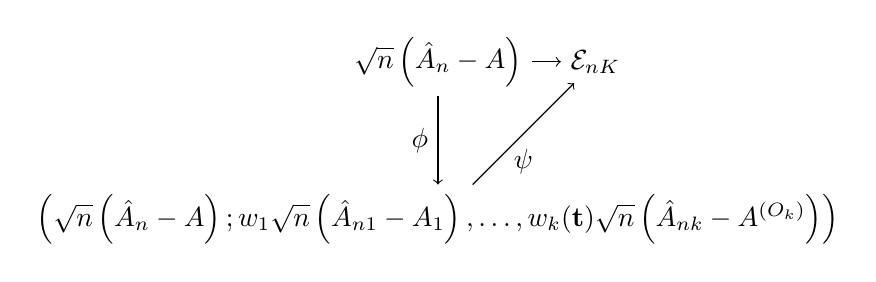
\begin{tikzpicture}[node distance=2cm, auto]
				\node (A) {$\sqrt{n}\left(\hat{A}_n - A\right)$};
				\node(B) [right of=A] {$\mathcal{E}_{nK}$};
				\node (C) [below of=A] {$\left(\sqrt{n}\left(\hat{A}_n - A\right) ; w_1\sqrt{n}\left(\hat{A}_{n1} - A_{1}\right), \dots, w_k(\textbf{t})\sqrt{n}\left(\hat{A}_{nk} - A^{(O_k)}\right)\right)$};	
				\draw[->](A) to node {}(B);
				\draw[->](A) to node [left] {$\phi$}(C);
				\draw[->](C) to node [below=0.5ex] {$\psi$}(B);
			\end{tikzpicture}
			\caption{Diagram of composition of function.}
			\label{fig:diagram}
		\end{figure}
	\end{proof}
	
	We now present all tools used obtain the exact recovery of our algorithm, that is $\hat{O} = \bar{O}$. The result is obtained by induction on step $l$ while we assume that the algorithm remains consistent at this step. If the algorithm wants to recover the first cluster $\bar{O}_1$ say, at step $l-1$ with an estimator $\hat{O}_1 \subset \bar{O}_1$ of size $|\hat{O}_1| = s_1 \leq d_1$. Take $j \in S \setminus \hat{O}_1$, we show that under conditions \eqref{eq:condition_consistent_recovery} and the cluster separation condition, that is $A^{(\bar{O}_1)} \in \mathcal{A}(\eta_{s_1+1})$, we have that :
	\begin{equation*}
		j \in \bar{O}_1 \quad \Longleftrightarrow \quad \widehat{SECO}(\hat{O}_1, j) > \alpha_{s_1+1}.
	\end{equation*}
	And thus the algorithm remains consistent at step $l$.
	
	\begin{proof}[Proof of Proposition \ref{prop:exact_recovery}]
		Without loss of generality, take $\bar{O}_1$ and we will show under conditions \eqref{eq:condition_consistent_recovery} and the separation condition, our algorithm remain consistent with any size of $\hat{O}_1$. Suppose without loss of generality that $\hat{O}_1 = \{i_{1,1}\}$ and thus $|\hat{O}_1| = 1$. Consider $j \in S \setminus \hat{O}_1$. We then observe that $j \notin \bar{O}_1 \implies SECO(\hat{O}_1,j) = 0$, and thus
		\begin{equation*}
			\widehat{SECO}(\hat{O}_1,j) \leq 2 \tau_2.
		\end{equation*}
		When the group separation at size $s_1 = 1$ holds, that is $A^{(O_1)} \in \mathcal{A}(\eta_2)$, we have that 
		\begin{equation*}
			j \in \bar{O}_1 \implies SECO(\hat{O}_1, j) > 4 \tau_2 \implies \widehat{SECO}(\hat{O}_1,j) > 2 \tau_2.
		\end{equation*}
		In particular, we have
		\begin{equation*}
			j \in \bar{O}_1 \quad \Longleftrightarrow \quad \widehat{SECO}(\hat{O}_1,j) > \alpha_2.
		\end{equation*}
		And the algorithm is consistent when $|\hat{O}_1| = 1$. Now we consider the algorithm at some step $l-1$ and assume that the algorithm was consistent up to this step, \emph{i.e.} $\hat{O}_1 \subset \bar{O}_1$ with $|\hat{O}_1| = s_1 \leq d_1$. Consider $j \in S \setminus \hat{O}_1$, at this step, we have :
		\begin{equation*}
			j \notin \bar{O}_1 \implies SECO(\hat{O}_1,j) = 0 \implies \widehat{SECO}(\hat{O}_1, j) \leq 2 \tau_{s_1+1}.
		\end{equation*}
		Under the group separation condition $A^{(O_1)} \in \mathcal{A}(\eta_{s_1+1})$, we obtain that
		\begin{equation*}
			j \in \bar{O}_1 \implies SECO(\hat{O}_1,j) > 4 \tau_{s_1+1} \implies \widehat{SECO}(\hat{O}_1, j) > 2 \tau_{s_1+1}.
		\end{equation*}
		Thus, under conditions \eqref{eq:condition_consistent_recovery} and the group separation condition, we have
		\begin{equation*}
			j \in \bar{O}_1 \quad \Longleftrightarrow \quad \widehat{SECO}(\hat{O}_1,j) > \alpha_{s_1+1}.
		\end{equation*}
		Thus, the algorithm remains consistent at step $l$ and exact recovery of the first cluster follows by induction.
		
		Now, exact recovery of all cluster follows also by induction. For $K = 1$, the result is given below. Suppose that at some step $K-1$, the algorithm was consistent up to this step, that is $\hat{O}_j = \bar{O}_j$ for every $j \in \{1,\dots,K\}$. Proceeding as below for the fist cluster, under conditions \eqref{eq:condition_consistent_recovery} and the separation condition, we obtain
		\begin{equation*}
			\hat{O}_{K} = \bar{O}_K,
		\end{equation*}
		and the proposition follows by induction.
	\end{proof}
	
	By denoting by $ALG$, the set of $U \subseteq \{1,\dots,d\}$ such that $|U| = s$ with $s \in \{1,\dots, d-1\}$ and $U$ is used by the split function, we will prove that Proposition \ref{prop:exact_recovery} holds with high probabilty for given parameters. Indeed, by Theorem 1, we know that $|ALG| \leq d^3$. We thus need to specify some threshold $\tau_s$ such that $|\hat{\theta}_n^{(U)} - \theta^{(U)}| \leq \tau_s$ with high probability. To do so, we make use of concentration inequality stated in Proposition \ref{prop:concentration_inequality} that gives concentration of an estimator of the extremal coefficient for a given size.
	
	\begin{proof}[Proof of Corollary \ref{corr:exact_recovery}]
		Following the notation introduced below, we have that for $t>0$ :
		\begin{equation*}
			\mathbb{P}\left\{ \bigcup_{U \in ALG} |\hat{\theta}_n^{(U)} - \theta^{(U)}| \geq t \right\} \leq \sum_{U \in ALG} \mathbb{P}\left\{|\hat{\theta}_n^{(U)} - \theta^{(U)}| \geq t \right\}.
		\end{equation*}
		Using Proposition \ref{prop:concentration_inequality}, one has 
		\begin{equation*}
			\mathbb{P}\left\{|\hat{\theta}_n^{(U)} - \theta^{(U)}| \geq t \right\} \leq 4 s \exp \left\{-\frac{nt^2}{128 s^2} \right\},
		\end{equation*}
		where $|U| = s$. By considering $\delta \in ]0,1[$ and solve the following equation
		\begin{equation*}
			\frac{\delta}{d^3} = 4 s \exp \left\{-\frac{nt^2}{128 s^2} \right\},
		\end{equation*}
		with respect to $t$ gives that :
		\begin{equation*}
			\mathbb{P}\left\{ \bigcup_{U \in ALG} |\hat{\theta}_n^{(U)} - \theta^{(U)}| \geq 8 s \sqrt{\frac{2}{n} \ln \left( \frac{2s d^3}{\delta} \right)} \right\} \leq \delta.
		\end{equation*}
		Now, taking $\delta = 4d^{-3A}$, we have that for every $U \in ALG$
		\begin{equation*}
			|\hat{\theta}_n^{(U)} - \theta^{(U)}| \leq 8 s \sqrt{\frac{2(1+A)}{n} \ln \left(s^{\frac{1}{1+A}} d \right)},
		\end{equation*}
		with probability higher than $1 - d^{-3A}$. The result then follows from Proposition \ref{prop:exact_recovery}, since for every $s \in \{1, \dots, d-1\}$, $\tau_{s} \leq 8 s \sqrt{\frac{2(1+A)}{n} \ln \left(s^{\frac{1}{1+A}} d \right)}$ with probability higher than $1-d^{-3A}$.
	\end{proof}
	
	\section{Proofs of auxiliary results}
		\subsection{extreme-value copula}
        
        In this first lemma, we prove that the function introduced in Paragraph 2.2 is indeed an extreme-value copula. For the ease of reading, we recall here its definition
        \begin{align*}
			\begin{array}{lrcl}
C_{\Pi} : & [0,1]^d & \longrightarrow & [0,1] \\
    & \textbf{u} & \longmapsto & \Pi_{k=1}^K C^{(k)}(u_{i_{k,1}}, \dots, u_{i_{k,d_k}}). \end{array}
		\end{align*}
		To prove this statement, we show that each margins is indeed distributed uniformly on the unit segment $[0,1]$. Hence $C$ is a copula function. In order to prove that $C$ is an extreme-value copula, we show that $C$ is max-stable as it is a characterizing property of extreme-value copula or, more generally, of extreme-value distribution.
	\begin{proof}[Proof of Lemma \ref{lem:Cevt}]
		We first show that $C$ is a copula function. It is clear that $C(\textbf{u}) \in [0,1]$ for every $\textbf{u} \in [0,1]^d$. We check that its univariate marginals are uniformly distributed on $[0,1]$. Without loss of generaly, take $u_{i_{1,1}} \in [0,1]$ and let us compute 
		\begin{equation*}
			C(1, \dots, u_{i_{1,1}}, \dots, 1) = C^{(1)}(u_{i_{1,1}}, 1, \dots, 1) \Pi_{k=1}^K C^{(k)}(1,\dots,1) = C^{(1)}(u_{i_{1,1}}, 1, \dots, 1) = u_{i_{1,1}}.
		\end{equation*}
		So $C$ is a copula function. We now have to prove that $C$ is an extreme-value copula. We recall that $C$ is an extreme-value copula if and only if $C$ is max-stable, that is for every $m \geq 1$
		\begin{equation*}
			C(u_1,\dots, u_d) = C(u_1^{1/m}, \dots, u_d^{1/m})^m.
		\end{equation*}
		By definition, we have
		\begin{equation*}
			C(u_1^{1/m}, \dots, u_d^{1/m})^m = \left( \Pi_{k=1}^K C^{(k)}\left(u_{i_{k,1}}^{1/m}, \dots, u_{i_{k,d_k}}^{1/m}\right) \right)^m = \Pi_{k=1}^K  \left\{ C^{(k)}\left(u_{i_{k,1}}^{1/m}, \dots, u_{i_{k,d_k}}^{1/m}\right) \right\}^m.
		\end{equation*}
		Using that $C^{(1)}, \dots, C^{(K)}$ are extreme-value copulae, thus max stable, we obtain
		\begin{equation*}
			C(u_1^{1/m}, \dots, u_d^{1/m})^m = \Pi_{k=1}^K C^{(k)}\left(u_{i_{k,1}}, \dots, u_{i_{k,d_k}}\right) = C(u_1, \dots, u_d).
		\end{equation*}
		Thus $C$ is an extreme-value copula. We end the proof by proving that $C$ is associated to the random vector $\textbf{X} = (\textbf{X}^{(1)}, \dots, \textbf{X}^{(K)})$, that is
		\begin{equation*}
			\mathbb{P} \left\{ \textbf{X} \leq \textbf{x} \right\} = C(G_1(x_1), \dots, G_d(x_d)), \quad \textbf{x} \in \mathbb{R}^d.
		\end{equation*}
		Using mutual independence between random vectors, we have
		\begin{align*}
			\mathbb{P}\left\{ \textbf{X} \leq \textbf{x} \right\} &= \Pi_{k=1}^K \mathbb{P}\left\{ X_{i_{k,1}} \leq x_{i_{k,1}}, \dots, X_{i_{k,d_k}} \leq x_{i_{k,d_k}} \right\} \\ &= \Pi_{k=1}^K C^{(k)}\left(G_{i_{k,1}}(x_{i_{k,1}}), \dots, X_{i_{k,d_k}} \leq x_{i_{k,d_k}} \right) \\ &= C(G_1(x_1), \dots, G_d(x_d)).
		\end{align*}
		Hence the result.
	\end{proof}
	
	\subsection{Proof of proposition \ref{prop:concentration_inequality}}
	\label{subsec:proof_concent_ineq}
	Technical details of this proof will be subdivised in some lemmas of which the combined use will gives the statement of Proposition \ref{prop:concentration_inequality}. The first lemma gives an upper bound of $|\hat{\theta}_n - \theta|$ with respect to $|\hat{\nu}_n(d^{-1},\dots, d^{-1}) - \nu(d^{-1},\dots, d^{-1})|$. This follows from the link between the Pickands dependence function and the madogram.
	\begin{lemma}
		\label{lem:upper_bounds_ext_coeff}
		We have,
		\begin{equation*}
			|\hat{\theta}_n - \theta| \leq 4 d |\hat{\nu}_n(d^{-1},\dots,d^{-1}) - \nu(d^{-1},\dots,d^{-1}) |.
		\end{equation*}
	\end{lemma}
	\begin{proof}
		Fix $\textbf{t} \in \Delta_{d-1}$, remember that $A(\textbf{t}) = f(\nu(\textbf{t}))$ and $\hat{A}_n(\textbf{t}) = f(\hat{\nu}_n(\textbf{t}))$, where $f :\mathbb{R}_+ \rightarrow \mathbb{R}_+, x \mapsto (x + c(\textbf{t})) / (1 - x - c(\textbf{t}))$ for every $\textbf{t} \in \Delta_{d-1}$ and $c(\textbf{t})$ is a constant equals to $d^{-1} \sum_{j=1}^d t_j / (1+t_j)$. Using that $A(\textbf{t}) \leq 1$, we have that
		\begin{equation*}
			\nu(\textbf{t}) + c(\textbf{t}) \leq 1 - \nu(\textbf{t}) - c(\textbf{t}).
		\end{equation*}
		We obtain that
		\begin{equation*}
			\nu(\textbf{t}) \leq \frac{1}{2} - c(\textbf{t}) < 1 - c(\textbf{t}).
		\end{equation*}
		In particular $1 - \nu(\textbf{t}) - c(\textbf{t}) \geq 2^{-1} > 0$. Now, taking derivation, we directly have for every $x \in [0, 2^{-1}-c(\textbf{t})]$
		\begin{equation*}
			|f'(x)| = \frac{1}{(1-x - c(\textbf{t}))^2} \leq 4.
		\end{equation*}
		Thus, $f$ is $4$-Lipschitz on $[0, 1-c(\textbf{t})]$ and in particular for $\textbf{t} = (d^{-1}, \dots, d^{-1})$
		\begin{equation*}
			|\hat{A}_n(d^{-1},\dots,d^{-1}) - A(d^{-1}, \dots, d^{-1})| \leq 4 |\hat{\nu}_n(d^{-1},\dots, d^{-1}) - \nu(d^{-1},\dots, d^{-1})|
		\end{equation*}
		Multiply by $d$ gives the statement.
	\end{proof}
	
	Now, we state a concentration inequality for the madogram estimator. This inequality is obtained through two main arguments, that are Hoeffding's inequality and the DKW inequality bound.
	
	\begin{lemma}
		\label{lem:mado_concent}
		For $t > 0$ and a fixed $\textbf{t} \in \Delta_{d-1}$, one has
		\begin{equation*}
			\mathbb{P}\left\{ |\nu_n(\textbf{t}) - \nu(\textbf{t}) | > t \right\} \leq 4 d \exp \left\{ -\frac{n t^2}{8} \right\}.
		\end{equation*}
	\end{lemma}
	\begin{proof}
		observe that
		\begin{equation*}
			|\hat{\nu}_n(\textbf{t}) - \nu(\textbf{t})| \leq |\hat{\nu}_n(\textbf{t}) - \nu_n(\textbf{t}) | + |\nu_n(\textbf{t}) - \nu(\textbf{t}) |,
		\end{equation*}
		where
		\begin{equation*}
			\nu_n(\textbf{t}) := \sum_{i=1}^n Y_i = \sum_{i=1}^n \frac{1}{n} \left[ \bigvee_{j=1}^d \left\{ F_j(X_{i,j}) \right\}^{1/t_j} - \frac{1}{d} \sum_{j=1}^d \left\{ F_j(X_{i,j}) \right\}^{1/t_j} \right].
		\end{equation*}
		As the following inequalities holds for every $i \in \{1,\dots,n\}$
		\begin{equation*}
			Y_i \leq \frac{(d-1)}{dn}.
		\end{equation*}
		Hoeffding's inequality applies and we obtain that
		\begin{equation*}
			\mathbb{P}\left\{ |\nu_n(\textbf{t}) - \nu(\textbf{t}) | > t / 2 \right\} \leq 2 \exp\left( - \frac{n d^2 t^2}{4(d-1)^2} \right).
		\end{equation*}
		Furthermore, we have 
		\begin{equation*}
			|\hat{\nu}_n(\textbf{t}) - \nu_n(\textbf{t}) | \leq 2 \underset{j \in \{1,\dots,d\}}{\sup}\underset{i \in \{1,\dots,n\}}{\sup} \left|\left\{ \hat{F}_{n,j}(X_{i,j}) \right\}^{1/t_j}- \left\{ F_{j}(X_{i,j}) \right\}^{1/t_j} \right|
		\end{equation*}
		Applying DKW inequality, we obtain
		\begin{equation*}
			\mathbb{P}\left\{ \underset{j \in \{1,\dots,d\}}{\sup}\underset{i \in \{1,\dots,n\}}{\sup} \left|\left\{ \hat{F}_{n,j}(X_{i,j}) \right\}^{1/t_j}- \left\{ F_{j}(X_{i,j}) \right\}^{1/t_j} \right|> \frac{t}{4}\right\} \leq 2d \exp\left( \frac{-nt^2}{8} \right).
		\end{equation*}
		We thus have for $d \geq 2$
		\begin{equation*}
			\mathbb{P}\left\{ \left| \hat{\nu}_n(\textbf{t}) - \nu(\textbf{t}) \right| > t \right\} \leq 4d\exp\left(- \frac{n t^2}{8} \right).
		\end{equation*}
		Hence the statement.
	\end{proof}
	
	Combine Lemma \ref{lem:upper_bounds_ext_coeff} and Lemma \ref{lem:mado_concent} gives Proposition \ref{prop:concentration_inequality}.
	
	\subsection{Asymptotic independence between multivariate extreme distribution}
	\label{subsec:asympto_indep}
	In this subsection, we extend the result given in Theorem 2.1 of \cite{takahashi1994asymptotic} for asymptotic independence between extreme random vector. The used arguments are similar of those used in the proof in \cite{takahashi1994asymptotic}. We make extensive use of the following result (see, for example \cite{10.1214/aop/1176993666} and the proof of Theorem 5.3.1 of \cite{galambos1978asymptotic}) \emph{i.e.} $F \in D(G)$ is equivalent to
	\begin{equation}
		\label{eq:app_galambos}
		\underset{n \rightarrow \infty}{\lim} \, n \left\{ 1 - F(\textbf{a}_n \textbf{x} + \textbf{b}_n) \right\} = - \ln G(\textbf{x})
	\end{equation}
	for all $\textbf{x}$ such that $0<G(\textbf{x}) <1$. In this section, we denote by $\bar{F}$ the survival function of $F$.
	
	\begin{theorem}
		\label{thm:ext_takahashi}
		Let $F$ be a $d$-distribution function and let $G^{(O_i)}$ be a $d_i$-extreme-value distribution for $i = 1,2$. Then for $\textbf{a}_n > 0$ and $\textbf{b}_n \in \mathbb{R}^d$
		\begin{equation}
			\label{eq:app_product}
			\left\{ F(\textbf{a}_n \textbf{x} + \textbf{b}_n) \right\}^n \underset{n \rightarrow \infty}{\longrightarrow} G^{(O_1)}(\textbf{x}^{(O_1)}) G^{(O_2)}(\textbf{x}^{(O_2)})
		\end{equation}
		if and only if
		\begin{equation}
			\label{eq:app_weak_conv}
			\left\{ F^{(O_i)} (\textbf{a}_n^{(O_i)} \textbf{x}^{(O_1)} + b_n^{(O_i)}) \right\}^{n} \underset{n \rightarrow \infty}{\longrightarrow} G^{(O_i)}(\textbf{x}^{(O_i)}),
		\end{equation}
		and there exists a $\textbf{p} = (\textbf{p}^{(O_1)}, \textbf{p}^{(O_2)}) \in \mathbb{R}^d$ such that $0 < H^{(O_1)}(\textbf{x}^{(O_1)}), H^{(O_2)}(\textbf{x}^{(O_2)}) < 1$ and
		\begin{equation}
			\label{eq:app_product_onepoint}
			\left\{ F(\textbf{a}_n \textbf{x} + \textbf{b}_n) \right\}^n \underset{n \rightarrow \infty}{\longrightarrow} G^{(O_1)}(\textbf{p}^{(O_1)}) G^{(O_2)}(\textbf{p}^{(O_2)})
		\end{equation}
	\end{theorem}
	\begin{proof}
		The proof follows exactly the same lines as in Theorem 2.1 of \cite{takahashi1994asymptotic}. One substantial difference is emphasizes in Remark. 
		For any $\textbf{x} \in \mathbb{R}^d$, $0 < H^{(O_1)}(\textbf{x}^{(O_1)}), H^{(O_2)}(\textbf{x}^{(O_2)}) < 1$, there exists $s > 0$ such that $\{ H^{(O_1)}(\textbf{x}^{(O_1)}) \}^{1/s} > H^{(O_1)}(\textbf{p}^{(O_1)})$, $\{ H^{(O_2)}(\textbf{x}^{(O_2)}) \}^{1/s} > H^{(O_2)}(\textbf{p}^{(O_2)})$. By Equation \eqref{eq:app_weak_conv}
		\begin{equation*}
			\left\{ F^{(O_i)}\left(\textbf{a}_{\lfloor sn \rfloor}^{(O_i)} \textbf{x}^{(O_i)} + b_{\lfloor sn \rfloor}^{(O_i)} \right) \right\}^{sn} \underset{n \rightarrow \infty}{\longrightarrow} H^{(O_i)}(\textbf{x}^{(O_i)})
		\end{equation*}
		thus
		\begin{equation*}
			\left\{ F^{(O_i)}\left(\textbf{a}_{\lfloor sn \rfloor}^{(O_i)} \textbf{x}^{(O_i)} + b_{\lfloor sn \rfloor}^{(O_i)} \right) \right\}^{n} \underset{n \rightarrow \infty}{\longrightarrow} \left\{ H^{(O_i)}(\textbf{x}^{(O_i)}) \right\}^{1/s}.
		\end{equation*}
		Notice that
		\begin{align*}
			\mathbb{P}\left\{ \left[ \textbf{X}^{(O_1)} \leq \textbf{x}^{(O_1)}, \textbf{X}^{(O_2)} \leq \textbf{x}^{(O_2)} \right]^c \right\} &= \mathbb{P} \left\{ \left[\textbf{X}^{(O_1)} \leq \textbf{x}^{(O_1)} \right]^c \cup \left[\textbf{X}^{(O_2)} \leq \textbf{x}^{(O_2)} \right]^c \right\} \\
			&= \mathbb{P} \left\{ \left[\textbf{X}^{(O_1)} \leq \textbf{x}^{(O_1)} \right]^c \right\} + \mathbb{P} \left\{ \left[\textbf{X}^{(O_2)} \leq \textbf{x}^{(O_2)} \right]^c \right\} \\
			&- \mathbb{P} \left\{ \left[\textbf{X}^{(O_1)} \leq \textbf{x}^{(O_1)} \right]^c \cap \left[\textbf{X}^{(O_2)} \leq \textbf{x}^{(O_2)} \right]^c \right\}.
		\end{align*}
		We thus obtain 
		\begin{align*}
		\mathbb{P} \left\{ \left[\textbf{X}^{(O_1)} \leq \textbf{x}^{(O_1)} \right]^c \cap \left[\textbf{X}^{(O_2)} \leq \textbf{x}^{(O_2)} \right]^c \right\} & = \left[ 1-\mathbb{P} \left\{ \textbf{X}^{(O_1)} \leq \textbf{x}^{(O_1)} \right\} \right] + \left[ 1 - \mathbb{P} \left\{ \textbf{X}^{(O_2)} \leq \textbf{x}^{(O_2)} \right\} \right] \\ &- \left[ 1- \mathbb{P}\left\{ \textbf{X}^{(O_1)} \leq \textbf{x}^{(O_1)}, \textbf{X}^{(O_2)} \leq \textbf{x}^{(O_2)} \right\} \right].
		\end{align*}
		Using Equations \eqref{eq:app_weak_conv} and \eqref{eq:app_product_onepoint} we have, in joint hands, that
		\begin{align*}
		&n \left[ 1 - \mathbb{P}\left\{ \textbf{X}^{(O_i)} \leq \textbf{a}_n^{(O_i)} \textbf{p}^{(O_i)} + \textbf{b}_n^{(O_i)} \right\} \right] \underset{n \rightarrow \infty}{\longrightarrow} - \ln G^{(O_i)} (\textbf{p}^{(O_i)}), \quad i =1,2 \\
		&n \left[ 1 - \mathbb{P}\left\{ \textbf{X} \leq \textbf{a}_n \textbf{p} + \textbf{b}_n \right\} \right] \underset{n \rightarrow \infty}{\longrightarrow} - \ln G^{(O_1)} (\textbf{p}^{(O_1)})G^{(O_2)} (\textbf{p}^{(O_2)}).
		\end{align*}
		Thus,
		\begin{equation*}
			\mathbb{P} \left\{ \left[\textbf{X}^{(O_1)} \leq \textbf{a}^{(O_1)} \textbf{p}^{(O_1)} + \textbf{b}_n^{(O_1)} \right]^c \cap \left[\textbf{X}^{(O_2)} \leq \textbf{a}^{(O_2)} \textbf{p}^{(O_2)} + \textbf{b}_n^{(O_2)} \right]^c \right\} \underset{n \rightarrow \infty}{\longrightarrow} 0.
		\end{equation*}
		Using now that $\left\{ \textbf{X}^{(O_1)} > \textbf{x}^{(O_1)}, \textbf{X}^{(O_2)} > x^{(O_2)} \right\} \subset \left\{ [\textbf{X}^{(O_1)} \leq \textbf{x}^{(O_1)}]^c \cap [\textbf{X}^{(O_2)} \leq \textbf{x}^{(O_2)}]^c \right\}$, we obtain
		\begin{equation*}
			 n \bar{F}(\textbf{a}_n \textbf{p} + \textbf{b}_n) \underset{n \rightarrow \infty}{\longrightarrow} 0.
		\end{equation*}
		By $\textbf{q} \geq \textbf{p}$, we now have
		\begin{equation*}
			0 \leq n \bar{F}(\textbf{a}_n \textbf{q} + \textbf{b}_n) \leq n \bar{F}(\textbf{a}_n \textbf{p} + \textbf{b}_n) \underset{n \rightarrow \infty}{\longrightarrow} 0.
		\end{equation*}
		The rest of the proof is similar to \cite{takahashi1994asymptotic}.
	\end{proof}
	
	\begin{remark}
		\label{rmk:takahashi}
		When $d_1 = d_2 = 1$, we immediately have that :
		\begin{equation*}
			\mathbb{P} \left\{ X_1 > x_1, X_2 > x_2  \right\} = \left[ 1-\mathbb{P} \left\{ X_1 \leq x_1 \right\} \right] + \left[ 1 - \mathbb{P} \left\{ X_2 \leq x_2\right\} \right] - \left[ 1- \mathbb{P}\left\{ X_1 \leq x_1, X_2 \leq x_2 \right\} \right].
		\end{equation*}
		We immediately obtain that, under the same hypotheses of Theorem \ref{thm:ext_takahashi} that
		\begin{equation}
			\label{eq:app_takahashi}
			n \bar{F}(\textbf{a}_n \textbf{p} + \textbf{b}_n) \underset{n \rightarrow \infty}{\longrightarrow} 0.
		\end{equation}
		The arguments exposed in this remark are those used in the proof of Theorem 2.1 \cite{takahashi1994asymptotic}. In our work framework, we do not directly obtain \eqref{eq:app_takahashi} but we can upper bound this quantity with respect to an other which indeedly converges to $0$ as $n\rightarrow \infty$ in the framework of Theorem \ref{thm:ext_takahashi}.
		
	\end{remark}
\end{document}